\documentclass[a4paper,10pt]{article}
% Paquete para inclusi�n de gr�ficos.
\usepackage{graphicx}
% Paquete para definir el idioma usado.
\usepackage[spanish]{babel}
% Paquete para definir la codificaci�n del conjunto de caracteres usado
% (latin1 es ISO 8859-1).
\usepackage[latin1]{inputenc}
\usepackage{hyperref}
% Include the listings-package
\usepackage{listings}  
\usepackage{pdfpages}


% T�tulo principal del documento.
\title{	\ Trabajo Pr�ctico N� 0: Infraestructura B�sica}
% Informaci�n sobre los autores.
\author{	Sebastian Ripari, \textit{Padr�n Nro. 96453}\\
            \texttt{ sebastiandanielripari@hotmail.com }\\\\
            Cesar, \textit{Padr�n Nro. PONER_PADRON}\\
            \texttt{ PONER_MAIL }\\\\
			Pablo Sivori, \textit{Padr�n Nro. 84026] }\\
            \texttt{ sivori.daniel@gmail.com }\\\\               
            \texttt{\footnotesize 1� Entrega: 07/09/2017}\\
            \\\\\\\\\\\\\\\\\\
            \normalsize{2do. Cuatrimestre de 2017}\\ 
            \normalsize{66.20 Organizaci�n de Computadoras} \\
            \normalsize{Facultad de Ingenier�a, Universidad de Buenos Aires} \\}
       
\date{}

\begin{document}
% Inserta el t�tulo.
\maketitle
% quita el n�mero en la primer p�gina
\thispagestyle{empty}
% Resumen
\begin{abstract}
En el presente trabajo pr�ctico se describir�n todos los pasos y 
conclusiones relacionadas al desarrollo e implementaci�n de una versi�n en lenguaje C,
de la Criba de Erat�stenes.
\end{abstract}
\newpage{}
\tableofcontents
\newpage{}

\begin{flushleft}

\par\end{flushleft}
\section{{\normalsize Introducci�n}}

El objetivo del presente trabajo pr�ctico es familiarizarse con el emulador gxemul mediante la implementacion de un programa que nos devuelva por stdout o en un archivo de salida, los n�meros primos menores a un n�mero natural N el cu�l es ingresado por par�metro.


\section{{\normalsize Implementaci�n}}

\subsection{{\normalsize Lenguaje}}

Como lenguaje de implementaci�n se eligi� ANSI C
ya que el mismo permite una alta portabilidad entre diferentes plataformas. 
El desarrollo del programa se realiz� usando un editor de texto 
(gedit,vim, kwrite) y compilando los archivos fuente con 
\htmladdnormallink{GCC}{http://gcc.gnu.org/} que viene en linux.
Para compilar, ejecutar el siguiente comando:

\begin{tabbing}
------- \= ----- \= \kill
\> \textbf{\emph{\$ make}}\\ 
\end{tabbing}

\subsection {{\normalsize Descripci�n del programa}}

Por empezar tenemos un archivo llamado \texttt{erat.c} que con tiene la funcion
\texttt{main}, aqui lo primero que hacemos la validacion de los argumentos, mediante 
una funcion llamada \texttt{validarArgumentos}. Caso de ingresarse algo invalido 
el programa no continuara, y retornara un valor distinto de 0, osea un codigo de error. Caso contrario, 
se llama a la funcion \texttt{realizarAccion} y aqui comienza el procesamiento de calcular 
la cantidad de numeros primos, entre 2 y el numero \texttt{tope} ingresado. Basicamente lo que hacemos es 
crear un array que contiene todos los numeros entre 2 y el numero ingresado, el \texttt{tope}. 
y luego le aplicamos a este array el algoritmo de la Criba de Erastostenes, mediante la funcion \texttt{encontrarNumerosPrimos},
que en las posiciones del array donde no hay un numero primo setea un cero.
Para luego tomar este array desde una funcion que se llama \texttt{imprimirPorPantalla}, y aqui imprimir todos los numeros distintos
de cero, que son los primos.

\subsubsection {{\normalsize Errores posibles}}

\begin{enumerate}
\item Fuera de rango: Cuando se ingresa un numero menor o igual que 1. El programa retorna 1. 
\item Comando invalido: Cuando se invoca al programa con flags inexistentes o escritos de forma desordenada. El programa retorna 2.
\end{enumerate}

\subsection{{\normalsize Corridas de prueba }}

\begin{enumerate}
\item Caso N = -5
El programa no imprime nada y retorna el codigo de error 1.
\item Caso N = 1
El programa no imprime nada y retorna el codigo de error 1. 
\item Caso N = 10
El programa imprime: 2 3 5 7 y retorna el codigo de exito 0.
\item Caso N = 50
El programa imprime 2 3 5 7 11 13 17 19 23 29 31 37 41 43 47 y retorna el codigo de exito 0.
\item Caso N = 100
El programa imprime 2 3 5 7 11 13 17 19 23 29 31 37 41 43 47 53 59 61 67 71 73 79 83 89 97 y retorna el codigo de exito 0.  
\end{enumerate}

\newpage{}
\subsection{{\normalsize Corridas de pruebas}}
	Para correr las pruebas se debe ejecutar el comando make del directorio pruebas y se veran resultados como los de 
	a continuacion:
	\newline
	\begin{center}
		\includegraphics[width=110mm,height=80mm]{PONER GRAFICO}
	\end{center}	
	
\newpage
\section{{\normalsize El c�digo fuente, en lenguaje C}}

	\lstinputlisting[language=C, basicstyle=\tiny]{../main.c}	

\newpage
\newpage
\newpage

\section{{\normalsize El c�digo MIPS32 generado por el compilado}}

	\lstinputlisting[language={[x86masm]Assembler}, firstline=1, lastline=45, basicstyle=\small]{../main.s}
 
 
\newpage{}
\section{{\normalsize Conclusiones}}

\begin{enumerate}
\item Si bien lo solicitado por el programa no era excesivamente dif�cil,
la realizaci�n completa del TP llev� cierta dificultad al tener que
realizarlo en el contexto solicitado: alta portabilidad, desarrollo
en C, e informe hecho en LaTeX. 
\item En el primer caso la dificultad radicaba en tener configurado 
y funcionando el GXEmul dentro de un Linux, y lograr que en ambos casos 
el programa compile y corra sin problemas. 
\item Debido a nuestro desconocimiento con LaTeX, tuvimos que 
invertir tiempo en encontrar forma de realizar el presente documento 
de la manera m�s correcta posible 
\item En cuanto al trabajo grupal en si mismo, no hubo inconvenientes de
ning�n tipo ya que al ser el grupo relativamente chico y tener conocimiento
del manejo del versionado de un proyecto ante cambios ingresado por
los integrantes (por medio del GIT), la introducci�n de modificaciones
y correcciones fu� fluida. 
\end{enumerate}

\newpage
\section{{\normalsize Enunciado del trabajo practico}}

	%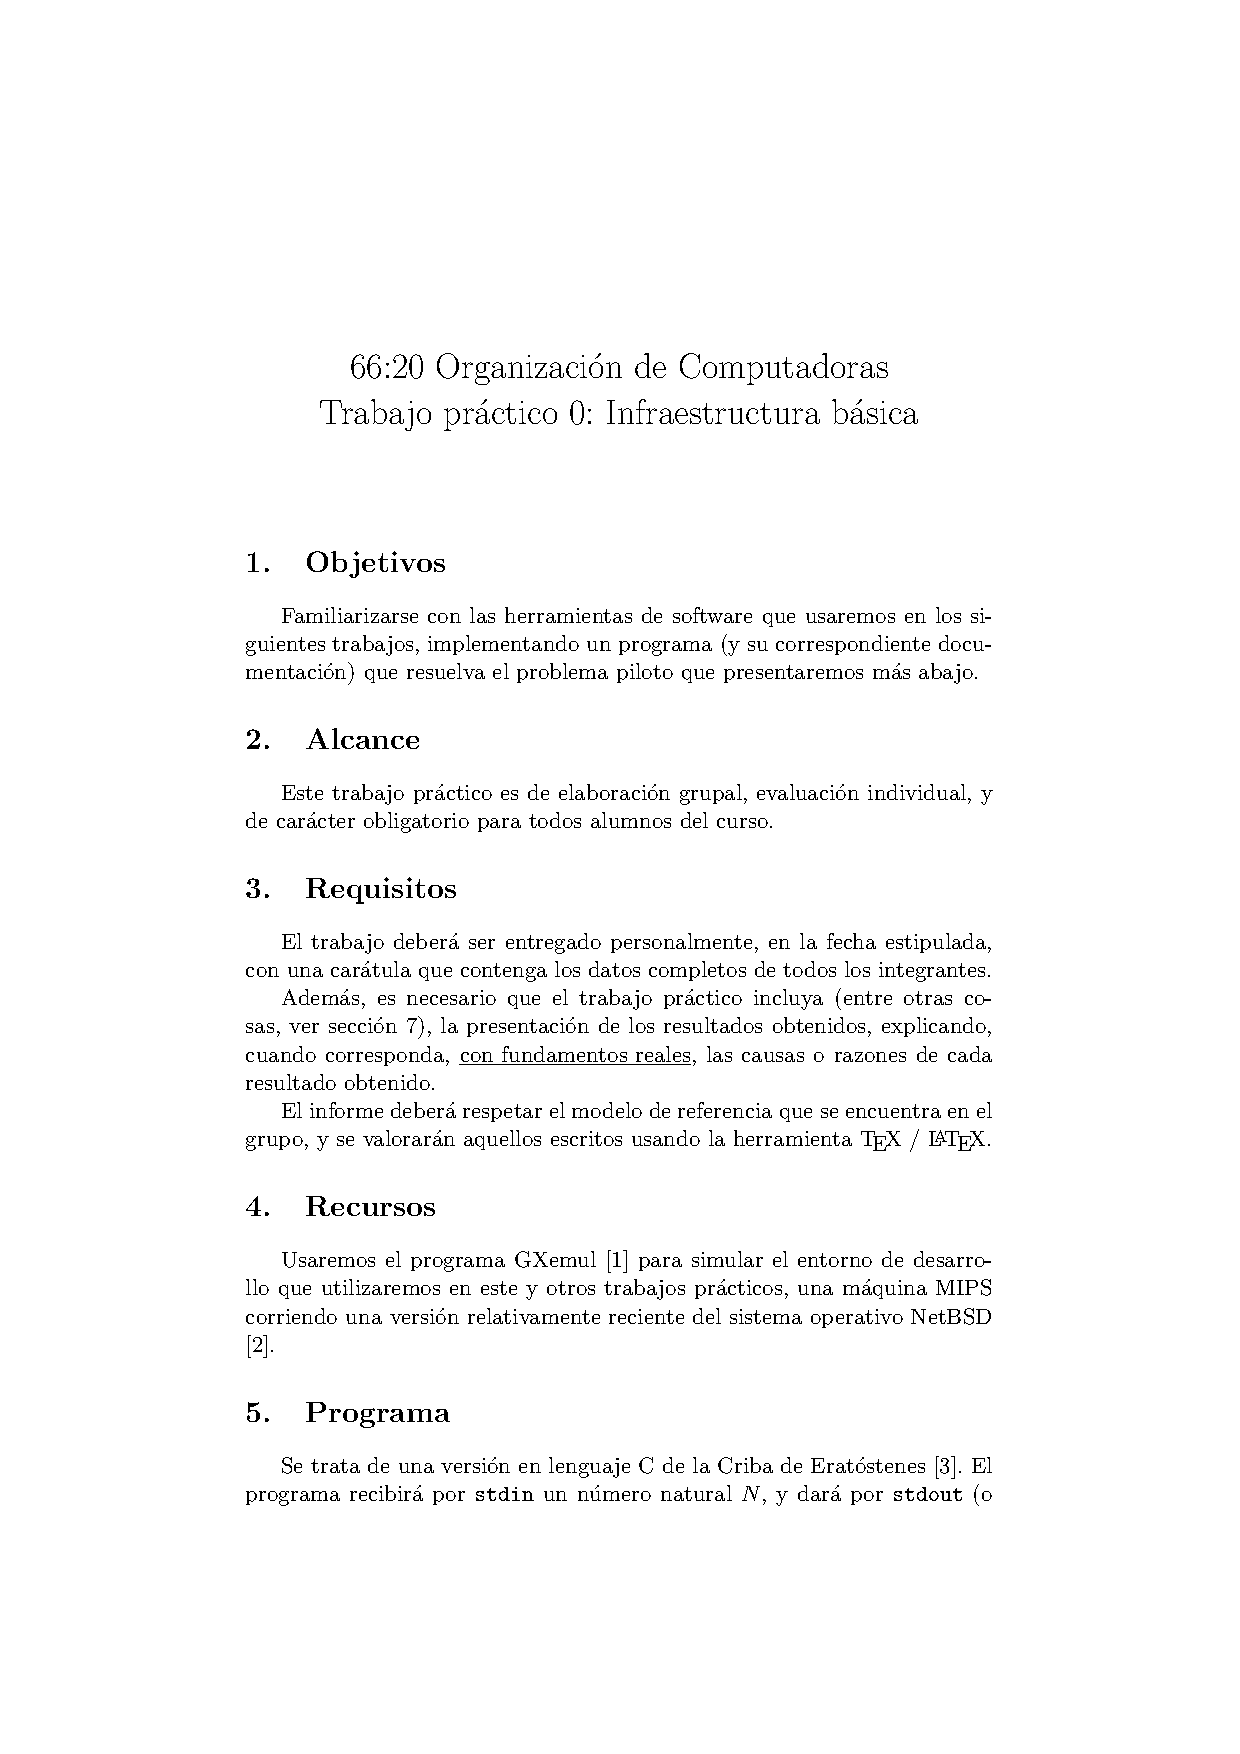
\includegraphics[width=0.8\textwidth]{enunciado.pdf}
	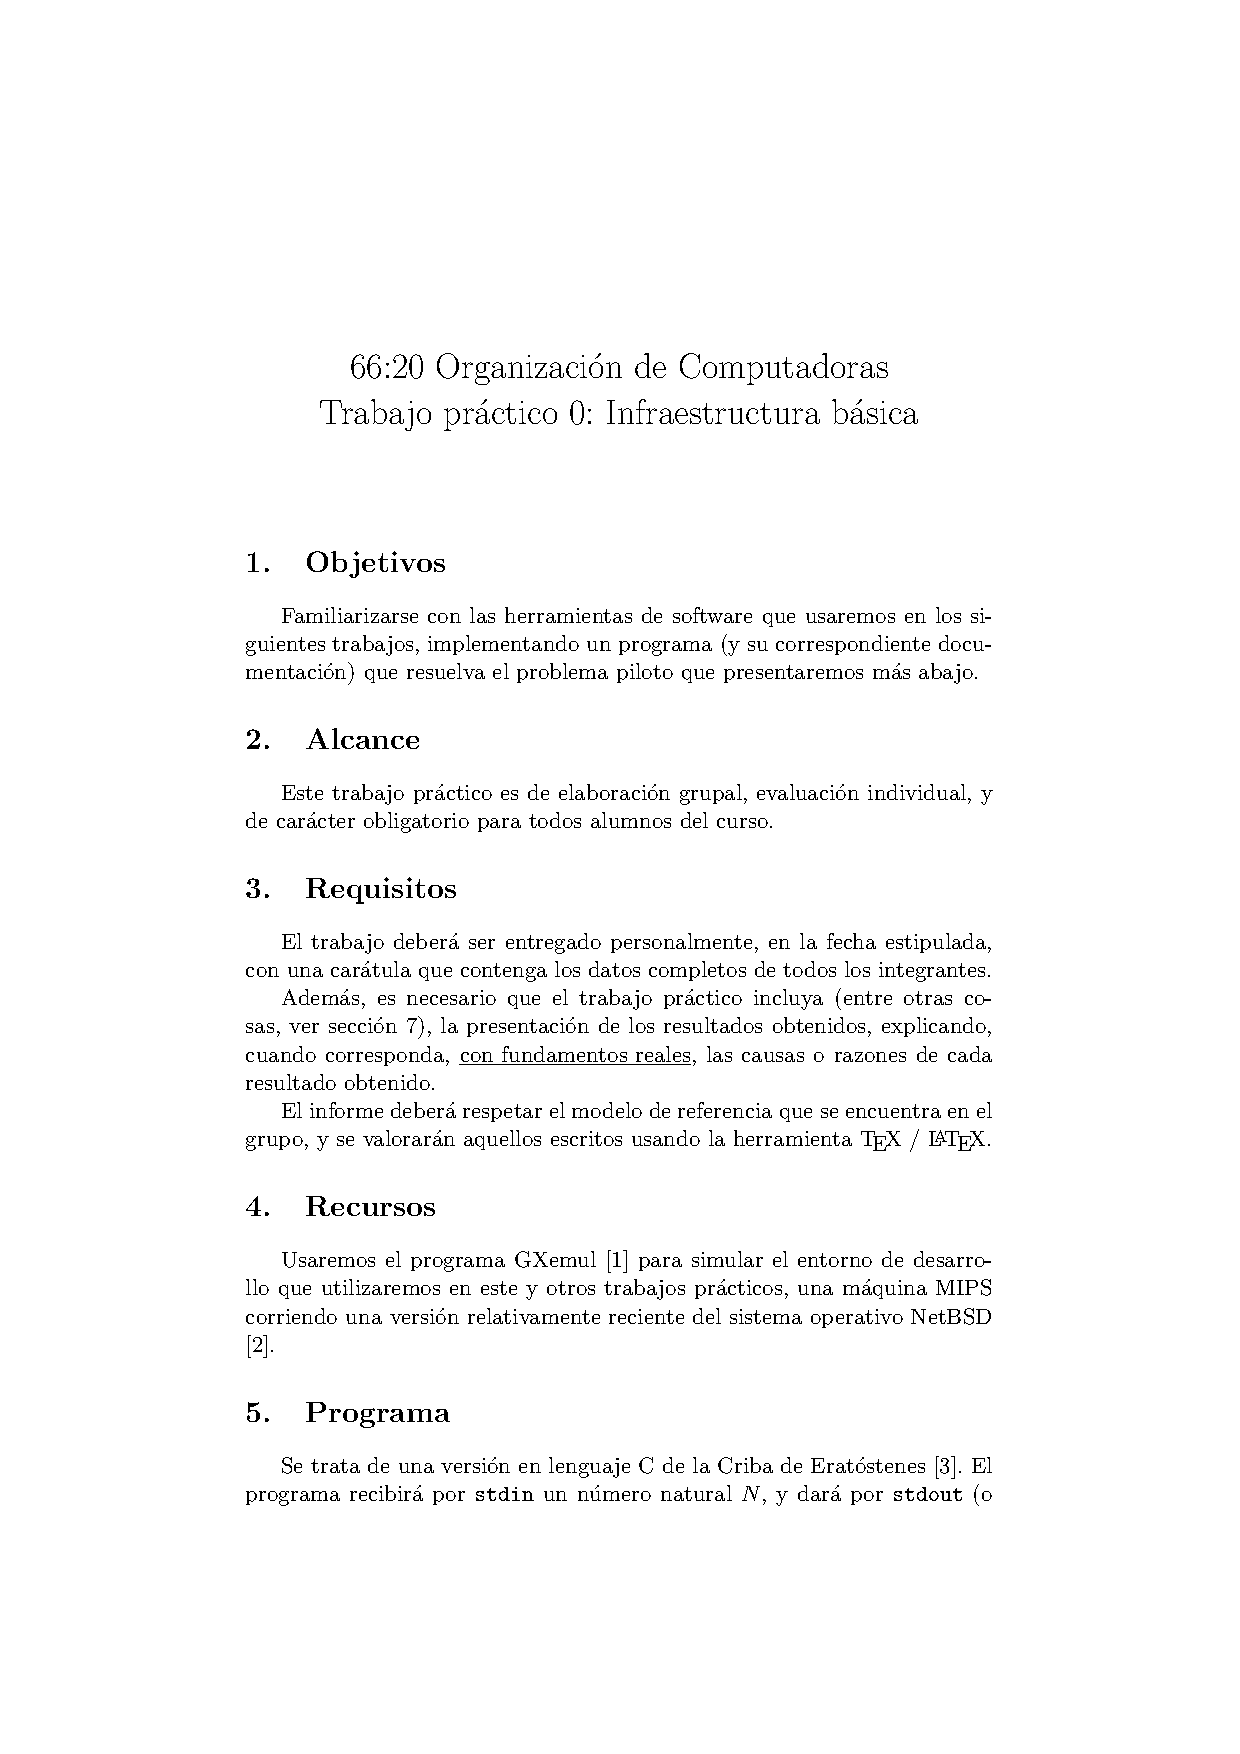
\includepdf[pages={1-},scale=0.75]{enunciado.pdf}


\bibliographystyle{plain}
\nocite{*}
\end{document}
